\chapter{Mitigate Fingerprinting of Honeypots}
\label{chap:fingerprinting}

\section{Fingerprinting Cowrie}

Attackers have a strong motivation to reveal honeypots before launching an attack.
Without any protection attackers would disclose their methods, and thus, newly developed attacks would become useless.
As shown in \autoref{chap:cloud-security}, attackers do try to get information about the host system.
\citet{vetterl2020} discussed various methods of fingerprinting, however, executing commands in a login shell and examining the response leaves precarious information to the honeypot itself.
In his work he evaluated methods to detect honeypots at the transport level.
As stated, the value of a honeypot would be merely zero if a detection on transport level would work.
He presents fingerprinting methods for SSH, Telnet, and HTTP/Web.
Due to the complexity of each method, we focus on SSH fingerprinting with the honeypot Cowrie.
The idea to detect SSH honeypots is to look for deviations in the response.
Therefore, \citet{vetterl2020} sends a set of probes $P = \{P_1, P_2, \dots, P_n\}$ to a given set of implementations of a network protocol $I = \{I_1, I_2, \dots, I_n\}$ and stores the set responses $R = \{R_1, R_2, \dots, R_n\}$.
For the given set of responses he calculated the cosine similarity coefficient $C$.
Goal is to find the best $P_i$ where the sum of $C$ is the lowest.
Cosine similarity helps to, it is widely used for text semantic similarity.

\begin{figure}[ht]
    \centering
    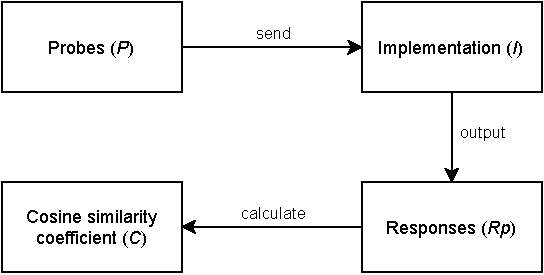
\includegraphics{figures/vetterl_concept.pdf}
    \caption[(derived from \cite{vetterl2020})]{Architecture of OpenSSH and Cowrie. OpenSSH and TwistedConch have subtle differences.}
    \label{fig:ss}
\end{figure}

%First, a set of SSH client version strings are created \verb| SSH-protoversion-swversion SP comment crlf| are created.
%Second, he creates \verb|SSH2_MSG_KEXINIT| packets using the algorithms defined in RFC 4250.
%Next, he calculates their cosine similarity coefficient to detect honeypots.
%In the beginning the best packet with the lowest cosine similarity coefficient $C$ has be defined.
In order to achieve that \citet{vetterl2020} created different SSH version strings.
In total, he used 
\verb|SSH2_MSG_KEXINIT| packets and compared their results.
The version string \verb|SSH-2.2-OpenSSH\r\n| and the \verb|SSH2_MSG_KEXINIT| packet including \textsc{ecdh-sha2-nistp521} as key-exchange algorithm, \textsc{ssh-dss} as host key algorithm, \textsc{blowfish-cbc} as encryption algorithm, \textsc{hmac-sha1} as mac algorithm and \textsc{zlib@openssh.com} as compression algorithm, with the wrong padding results in the lowest cosine similarity coefficient $C$

\begin{figure}[ht]
    \centering
    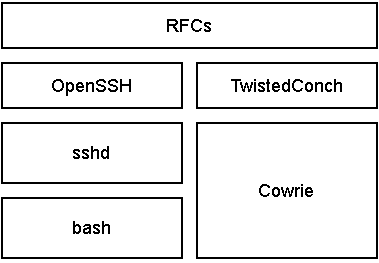
\includegraphics{figures/cowrie-openssh.pdf}
    \caption[Architecture of OpenSSH and Cowrie]{Architecture of OpenSSH and Cowrie. OpenSSH and TwistedConch have subtle differences.}
    \label{fig:cowrie-openssh}
\end{figure}

\citet{vetterl2020} states that current low- and medium-interaction honeypots have a generic weakness due to the underlying off-the-shelf libraries.
Cowrie is based on TwistedConch, a library that implements the SSH protocol.
Any bash response is implemented by Cowrie.
However, 

\section{Disguising Cowrie}

After 

\section{Experiment}

\begin{figure}
    \lstinputlisting[language=bash, caption={OpenSSH connection attempt with probed SSH packet}, label={lst:ssh-openssh}]{listings/ssh-openssh.txt}
\end{figure}

\begin{figure}
    \lstinputlisting[language=bash, caption={Cowrie connection attempt with probed SSH packet}, label={lst:ssh-cowrie}]{listings/ssh-cowrie.txt}
\end{figure}

\begin{figure}
    \lstinputlisting[language=bash, caption={Disguised Cowrie connection attempt with probed SSH packet}, label={lst:ssh-cowrie-fixed}]{listings/ssh-cowrie-fixed.txt}
\end{figure}

%So would it be ok if you take a picture of the IBM box inside the shipping box  with my delivery details and timestamp? And additionally, a picture of the sealed shipping box with the shipping note from DHL.
%I guess that would be sufficient for me.